\chapter{Демонстрационные примеры использования интегрированной среды и компилятора}\label{ch:ch4}

\section{Факториал}\label{sec:ch4/sect1}

На рисунке \ref{fig:fact_regular} представлена программа, вычисляющая факториал числа n как $0! = 1, n! = n(n - 1)!$

\begin{figure}[ht]
	\centering
	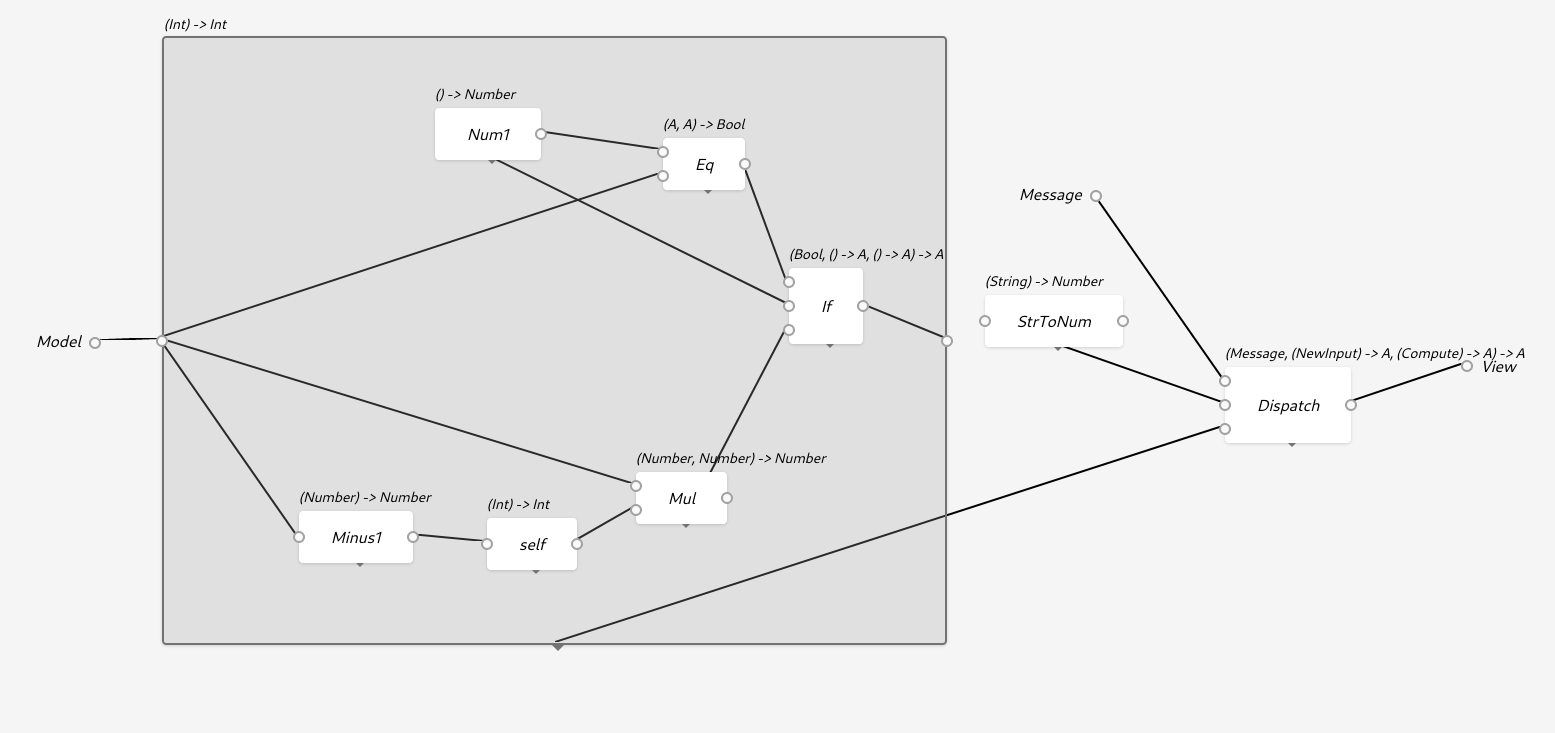
\includegraphics [scale=0.4] {fact_regular}
	\caption{Программа на Flovver, вычисляющая факториал}
	\label{fig:fact_regular}
\end{figure}

\FloatBarrier

Для программы генерируется следующий целевой код на JavaScript (опуская код примитивных функций и среды исполнения):

\begin{lstlisting}[language=JavaScript]
const update = (model, message) => {
    const fsa_1 = (fsa_1_arg_0) => StrToNum(fsa_1_arg_0);
    const fsa_2 = () => Num1();
    const fsa_6 = () => {
        const fsa_6_r = (fsa_6_arg_0) => {
            const fsa_7 = () => Minus1(fsa_6_arg_0);
            const fsa_8 = () => fsa_6_r(fsa_7());
            const fsa_9 = () => Mul(fsa_6_arg_0, fsa_8());
            const fsa_10 = () => Eq(fsa_2(), fsa_6_arg_0);
            const fsa_11 = () => If(fsa_10(), fsa_2, fsa_9);
            return fsa_11();
        }
        return fsa_6_r(model);
    }
    const fsa_12 = () => Dispatch(message, fsa_1, fsa_6);
    return fsa_12();
}
\end{lstlisting}

\FloatBarrier

\section{Оптимизация хвостовой рекурсии при вычислении факториала}\label{sec:ch4/sect2}

Факториал на Flovver в хвостово-рекурсивной форме представлен на рисунке \ref{fig:fact_tailrec}. 

\begin{figure}[ht]
	\centering
	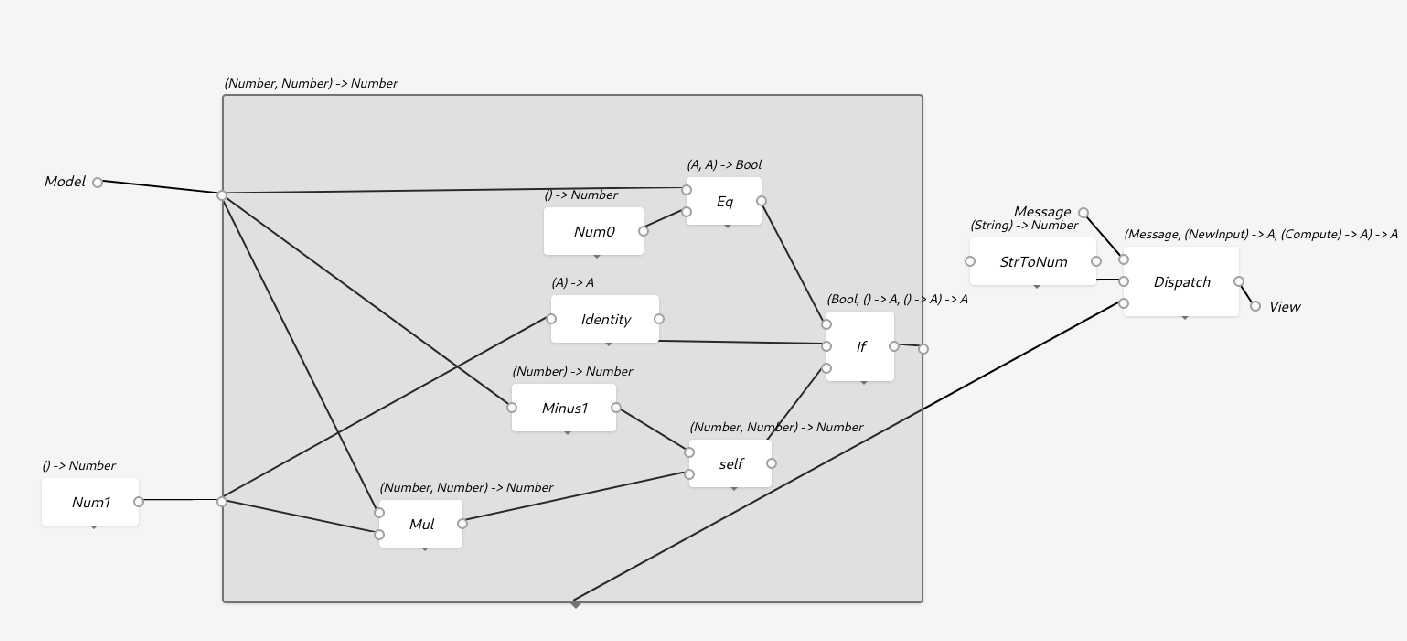
\includegraphics [scale=0.35] {fact_tailrec}
	\caption{Хвостово-рекурсивный факториал на Flovver}
	\label{fig:fact_tailrec}
\end{figure}

\FloatBarrier

С установленным флагом устранения хвостовой рекурсии, для программы генерируется следующий код:

\begin{lstlisting}[language=JavaScript]
const update = (model, message) => {
    const fsa_1 = (fsa_1_arg_0) => StrToNum(fsa_1_arg_0);
    const fsa_2 = () => Num0();
    const fsa_3 = () => Num1();
    const fsa_7 = () => {
        const fsa_7_r = (fsa_7_arg_0_i,fsa_7_arg_1_i) => {
            let [fsa_7_arg_0,fsa_7_arg_1] = [fsa_7_arg_0_i,fsa_7_arg_1_i];
            const fsa_8 = () => Mul(fsa_7_arg_0,fsa_7_arg_1);
            const fsa_9 = () => Eq(fsa_2(),fsa_7_arg_0);
            const fsa_10 = () => Identity(fsa_7_arg_1);
            const fsa_11 = () => Minus1(fsa_7_arg_0);
            const fsa_12 = () => Tail(fsa_7_r,fsa_11(),fsa_8());
            const fsa_13 = () => If(fsa_9(),fsa_10,fsa_12);
            while (true) {
                const result = fsa_13();
                if (IsTail(result)) {
                    [fsa_7_arg_0,fsa_7_arg_1] = result.parameters;
                    continue;
                }
                return result;
            }

        }
        return fsa_7_r(model,fsa_3());
    }
    const fsa_14 = () => Dispatch(message,fsa_1,fsa_7);
    return fsa_14();
}
\end{lstlisting}

\section{Функция Фибоначчи}\label{sec:ch4/sect3}

На рисунке \ref{fig:flovver_fib} представлена программа, вычисляющая функцию Фибоначчи
как $F_0 = 0,\quad F_1 = 1,\quad F_n = F_{n-1} + F_{n-2}$ при $n \ge 2$.

\begin{figure}[ht]
	\centering
	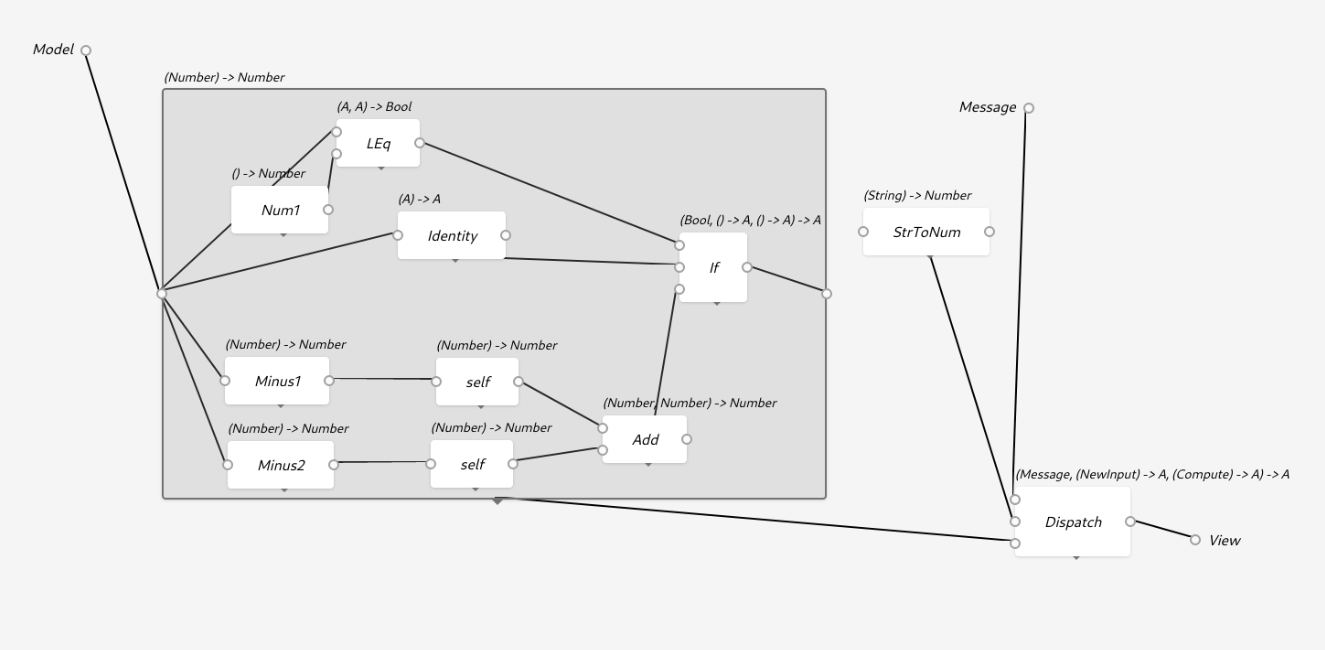
\includegraphics [scale=0.5] {flovver_fib}
	\caption{$F_n$ на Flovver}
	\label{fig:flovver_fib}
\end{figure}

\FloatBarrier

С выключенными флагами оптимизатора для программы генерируется следующий код:

\begin{lstlisting}[language=JavaScript]
const update = (model, message) => {
    const fsa_1 = () => Num1();
    const fsa_2 = (fsa_2_arg_0) => StrToNum(fsa_2_arg_0);
    const fsa_6 = () => {
        const fsa_6_r = (fsa_6_arg_0) => {
            const fsa_7 = () => Minus2(fsa_6_arg_0);
            const fsa_8 = () => fsa_6_r(fsa_7());
            const fsa_9 = () => Minus1(fsa_6_arg_0);
            const fsa_10 = () => fsa_6_r(fsa_9());
            const fsa_11 = () => Add(fsa_10(), fsa_8());
            const fsa_12 = () => Identity(fsa_6_arg_0);
            const fsa_13 = () => LEq(fsa_6_arg_0, fsa_1());
            const fsa_14 = () => If(fsa_13(), fsa_12, fsa_11);
            return fsa_14();
        }
        return fsa_6_r(model);
    }
    const fsa_15 = () => Dispatch(message, fsa_2, fsa_6);
    return fsa_15();
}
\end{lstlisting}

\section{Мемоизация функции Фибоначчи}\label{sec:ch4/sect4}

С установленным флагом мемоизации вычислений, для программы вычисления функции Фибоначчи
генерируется код вида:

\begin{lstlisting}[language=JavaScript]
const update = (model, message) => {
    const fsa_1 = () => Num1();
    const fsa_2 = (fsa_2_arg_0) => StrToNum(fsa_2_arg_0);
    const fsa_6 = () => {
        const fsa_6_r = (() => {
            const fsa_6_st = {};
            const fsa_6_w = (fsa_6_arg_0) => {
                const fsa_7 = () => Minus2(fsa_6_arg_0);
                const fsa_8 = () => fsa_6_r(fsa_7());
                const fsa_9 = () => Minus1(fsa_6_arg_0);
                const fsa_10 = () => fsa_6_r(fsa_9());
                const fsa_11 = () => Add(fsa_10(), fsa_8());
                const fsa_12 = () => Identity(fsa_6_arg_0);
                const fsa_13 = () => LEq(fsa_6_arg_0, fsa_1());
                const fsa_14 = () => If(fsa_13(), fsa_12, fsa_11);
                return fsa_14();
            }
            return (fsa_6_arg_0) => fsa_6_st[[fsa_6_arg_0]] = fsa_6_st[[fsa_6_arg_0]] || fsa_6_w(fsa_6_arg_0);
        })();
        return fsa_6_r(model);
    }
    const fsa_15 = () => Dispatch(message, fsa_2, fsa_6);
    return fsa_15();
}
\end{lstlisting}

\clearpage
